\documentclass{beamer}
% definitions for slides for the semantics course - CSC501
% Lutz Hamel, (c) 2006

\usetheme{Warsaw}
\usepackage{bussproofs}
\usepackage{amsmath}
\usepackage{amssymb}
\usepackage{latexsym}
\usepackage{xypic}
\usepackage{alltt}
\usepackage{rotating}
\usepackage{graphicx}
\usepackage{url}

\newcommand{\ul}[1]{\underline{#1}}
\newcommand{\orbar}{\,|\,}
\newcommand{\co}{\,\colon\;}
\newcommand{\syntaxset}[1]{\ensuremath{\mbox{\bf #1}}}
\newcommand{\nonterm}[1]{\ensuremath{\mbox{#1}}}
\newcommand{\term}[1]{\ensuremath{\mbox{\bf #1}}}
\newcommand{\ifstmt}[3]{\ensuremath{{\bf if}\; {#1}\;{\bf then}\;{#2}\;{\bf else}\;{#3}\;\term{end}}}
\newcommand{\whilestmt}[2]{\ensuremath{{\bf while}\; {#1}\;{\bf do}\;{#2}\; \term{end}}}
\newcommand{\funcstmt}[3]{\ensuremath{{\bf fun}\; {#1}\; {\bf is}\; {#2} \; {\bf return}\; {#3}}}
\newcommand{\localstmt}[1]{\ensuremath{{\bf local}\; {#1}}}
\newcommand{\pairmap}[3]{\ensuremath{( {#1}, {#2} ) \mapsto {#3}}}
\newcommand{\single}[1]{\ensuremath{\langle {#1}\rangle}}
\newcommand{\pair}[2]{\ensuremath{({#1}, {#2} )}}
\newcommand{\triple}[3]{\ensuremath{\langle {#1}, {#2}, {#3} \rangle}}
\newcommand{\cond}[3]{\ensuremath{({#1}?\,{#2} : {#3})}}
\newcommand{\condbar}[3]{\ensuremath{({#1}\rightarrow{#2} \mid {#3})}}
\newcommand{\sem}[2]{\ensuremath{{#1}-\!\!-\!\!\!\!\gg{#2}}}
\newcommand{\liftfunc}[1]{\ensuremath{\lfloor{#1}\rfloor}}
\newcommand{\bcode}{\begin{alltt}\scriptsize}
\newcommand{\ecode}{\end{alltt}}
\newcommand{\comment}[1]{}

\newcommand{\fframe}[1]{
\begin{center}
\fbox{
\begin{minipage}{3.6in}
{#1}
\end{minipage}
}
\end{center}
}

\begin{document}

%%%%%%%%%%%%%%%%%%%%%%%%%%%%%%%%%%%%%%%%%%%%%%%%
\begin{frame}{First-Order Logic}

The formal system of first-order logic is constructed around the idea of well-formed formulas (WFFs).
The simplest WFFs are,
\begin{itemize}
\item
{\bf Variables} are symbols used to represent unspecified objects or individuals. Variables are typically denoted by single lowercase letters (e.g., x, y,  z).\footnote{This only applies to pencil-and-paper logic. Prolog has its own rules in what constitutes a variable.}

\item
{\bf Constants} represent specific, fixed objects or individuals in the domain of discourse. 
The most well known constants are the Boolean constants $\mathit{true}$ and $\mathit{false}$.

\item
{\bf Predicates} are functions that represent properties or relations that can be true or false for individuals. Predicates are typically denoted by uppercase letters (e.g., P, Q, R) followed by a number of arguments. For example, P(x), Q(x, y), R(y, z, w) are predicates.\footnote{This notational convention again only applies to pencil-and-paper logic.}

\end{itemize}

\end{frame}



%%%%%%%%%%%%%%%%%%%%%%%%%%%%%%%%%%%%%%%%%%%%%%%%
\begin{frame}{First-Order Logic}

Connectives are used to form more complex formulas from simpler ones. 
The most common connectives in first-order logic are,
\begin{itemize}
\item
{\bf Negation ($\neg$):} 
Given a formula $A$, $\neg A$ represents the negation or the opposite of $A$.

\item
{\bf Conjunction ($\wedge$):}
Given two formulas $A$ and $B$, $A \wedge B$ represents the logical AND of $A$ and $B$.

\item
{\bf Disjunction ($\vee$):} 
Given two formulas $A$ and $B$, $A \vee B$ represents the logical OR of $A$ and $B$.

\item
{\bf Implication ($\rightarrow$):} 
Given two formulas $A$ and $B$, $A \rightarrow B$ represents the implication: if $A$ then $B$.
In the English grammar this can also be expressed as: $B$ if $A$.

\item
{\bf Equivalence ($\leftrightarrow$):}
Given two formulas $A$ and $B$, $A \leftrightarrow B$ represents the equivalence or "if and only if" statement between $A$ and $B$, often written as $A \mbox{ iff } B$.

\end{itemize}

\end{frame}

%%%%%%%%%%%%%%%%%%%%%%%%%%%%%%%%%%%%%%%%%%%%%%%%
\begin{frame}{First-Order Logic}

{\bf Quantifiers} are used to express statements about all or some individuals in the domain of discourse. Predicates and quantifiers as additions to modern logic are the contributions of 
Gottlob Frege, a logician and philosopher from the 19th  century.

\begin{center}
    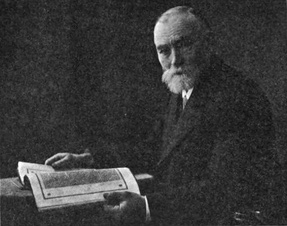
\includegraphics[height=15mm]{images/gottlob-frege}
\end{center}

The two main quantifiers in first-order logic are:
\begin{itemize}
\item
{\bf Universal Quantifier ($\forall$):} Given a variable $x$ and a formula $A(x)$, $\forall x [A(x)]$ represents ``for all $x$, $A(x)$ is $\mathit{true}$.''

\item
{\bf Existential Quantifier ($\exists$):} Given a variable $x$ and a formula $A(x)$, $\exists x [A(x)]$ represents ``there exists an $x$ such that $A(x)$ is $\mathit{true}$.''
\end{itemize}

\end{frame}

%%%%%%%%%%%%%%%%%%%%%%%%%%%%%%%%%%%%%%%%%%%%%%%%
\begin{frame}{WFFs}
Here are some example WFFs in first-order logic:
\begin{itemize}
\item
$\mathit{human}(\mathit{socrates})$ -- here $\mathit{human}$ is a predicate and $\mathit{socrates}$ is a constant.

\item
$\forall x[\mathit{human}(x) \rightarrow \mathit{mortal}(x)]$ -- $x$ is a variable and $\mathit{human}$ and
$\mathit{mortal}$ are predicates.

\item
$\forall x \exists y [\mathit{human}(x) \wedge \mathit{parent}(y,x)]$ -- here $\mathit{parent}(y,x)$ means
$y$ is the parent of $x$.

\item
$\forall x[\mathit{man}(x) \wedge \mathit{parent}(x)]$
\end{itemize}
\end{frame}


%%%%%%%%%%%%%%%%%%%%%%%%%%%%%%%%%%%%%%%%%%%%%%%%
\begin{frame}{Deduction}

We have seen that we can construct first-order logic sentences and we have an intuitive idea
on how to interpret them.\footnote{Logician are concerned about formal ways of assigning 
meaning to logic formulas -- model theory.}

\vspace{.1in}
The question now is, how do we reason using logic?
\begin{itemize}
\item Deduction!
\end{itemize}
Deduction or inference is process of deriving new sentences from existing ones.  
The kind of deduction one is allowed to make is defined by the notation and a set of inference rules.

\end{frame}

%%%%%%%%%%%%%%%%%%%%%%%%%%%%%%%%%%%%%%%%%%%%%%%%
\begin{frame}{Deduction}

Classical first-order logic has a quite a few deduction rules,\footnote{Source: ``Symbolic Logic'', I. Copi, Macmillian, 1979.}

\begin{center}
    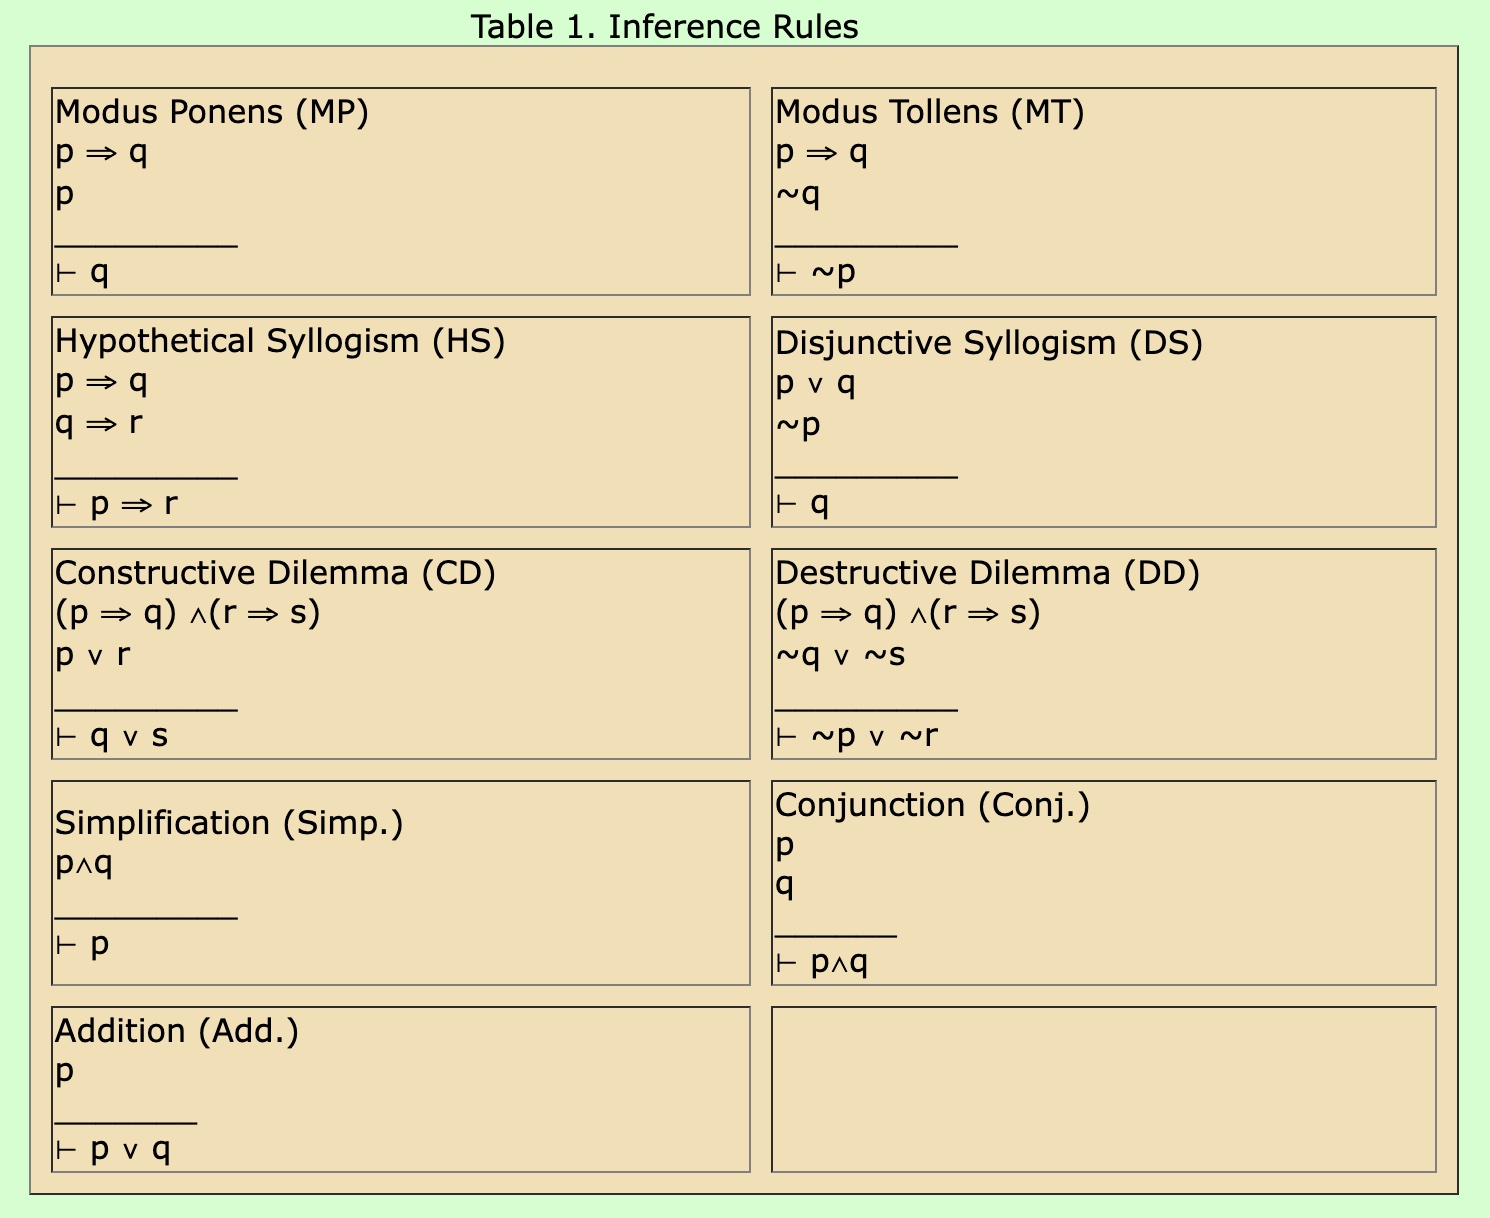
\includegraphics[height=60mm]{images/inference-rules}
\end{center}

{\bf Note:} The table uses $\Rightarrow$ as implication and $\sim$ as the logical not.

\end{frame}

%%%%%%%%%%%%%%%%%%%%%%%%%%%%%%%%%%%%%%%%%%%%%%%%
\begin{frame}{Deduction}
From our perspective the {\bf modus ponens} is the most important rule because
\begin{enumerate}
\item
It is the main inference rule on which our natural deduction system for our semantics is based on.

\item
It is the only inference rule implemented in Prolog.

\end{enumerate}

\vspace{.1in}
{\bf Example:} 
\[
\begin{array}{l}
\forall x[\mathit{human}(x) \rightarrow \mathit{mortal}(x)]\\
\mathit{human}(\mathit{socrates})\\ \hline
\therefore\mathit{mortal}(\mathit{socrates})
\end{array}
\]

\end{frame}

%%%%%%%%%%%%%%%%%%%%%%%%%%%%%%%%%%%%%%%%%%%%%%%%
\begin{frame}{A Word or Two about Implication}
The truth table for the implication operator `$\rightarrow$' can be given as (assuming $1\equiv \mathit{true}$ and $0\equiv\mathit{false}$)
{\scriptsize
\[
\begin{array}{lcc|c}
&A & B & A \rightarrow B\\ \hline
(1)& 1 & 0 & 0\\
(2) & 1 & 1 & 1\\
(3) & 0 & 0 & 1\\
(4) & 0 & 1 & 1
\end{array}
\]
}
Entries $(1)$ and $(2)$ are intuitive: When the antecedent $A$ is true but the consequent $B$ is false then
the implication itself is false.  If both the antecedent and the consequent are true then the implication is true.

\vspace{.1in}

However, entries $(3)$ and $(4)$ are somewhat counter intuitive.  They state that if the antecedent $A$ is false
then the implication is true regardless of the value of the consequent.  In other words, we can conclude ``anything''
from an antecedent that is false.  In mathematical jargon we say that $(3)$ and $(4)$  {\bf hold trivially}.
\end{frame}

%%%%%%%%%%%%%%%%%%%%%%%%%%%%%%%%%%%%%%%%%%%%%%%%
\begin{frame}{A Word or Two about Implication -- An Example}

{\scriptsize
\[
\begin{array}{l}
\mbox{If Bob is a bachelor, then he is single.}\\
\mbox{Bob is a bachelor.}\\ \hline
\therefore\mbox{Bob is single.}
\end{array}
\]
}
Now consider an antecedent that is not true,
{\scriptsize
\[
\begin{array}{l}
\mbox{If Bob is a bachelor, then he is single.}\\
\mbox{Bob is not a bachelor.}\\ \hline
\therefore\mbox{Bob is not single (by rule $(3)$).}
\end{array}
\]
}
Since the antecedent is not true rule $(3)$ allows us to conclude the
opposite of what the implication dictates.  However, the following is also
valid reasoning,
{\scriptsize
\[
\begin{array}{l}
\mbox{If Bob is a bachelor, then he is single.}\\
\mbox{Bob is not a bachelor.}\\ \hline
\therefore\mbox{Bob is  single (by rule $(4)$).}
\end{array}
\]
}
Not being a bachelor does not necessarily imply that Bob is not single.  For example,
Bob could be a widower or a divorcee.
\end{frame}

%%%%%%%%%%%%%%%%%%%%%%%%%%%%%%%%%%%%%%%%%%%%%%%%
\begin{frame}{A Word or Two about Implication}

Given the truth table for implication,
\[
\begin{array}{lcc|c}
&A & B & A \rightarrow B\\ \hline
(1)& 1 & 0 & 0\\
(2) & 1 & 1 & 1\\
(3) & 0 & 0 & 1\\
(4) & 0 & 1 & 1
\end{array}
\]
this means that in order to show that an implication holds we only have to show that rule $(2)$
holds.  Rule $(1)$ states that the implication is false and rules $(3)$ and $(4)$ are trivially true and
therefore not interesting.

\vspace{.1in}
{\bf Note:} We will see that in our approach to semantics (natural semantics) that is precisely what we aim to do!
\end{frame}

%%%%%%%%%%%%%%%%%%%%%%%%%%%%%%%%%%%%%%%%%%%%%%%%
\begin{frame}{Closely Related: Equivalence}

We write $A \leftrightarrow B$ if $A$ and $B$ are equivalent.

Given the truth table for the equivalence operator is given as,
\[
\begin{array}{lcc|c}
&A & B & A \leftrightarrow B\\ \hline
(1)& 1 & 0 & 0\\
(2) & 1 & 1 & 1\\
(3) & 0 & 0 & 1\\
(4) & 0 & 1 & 0
\end{array}
\]
That is, the operator only produces a true value if $A$ and $B$ have the same truth assignment.

Another, and very useful, way to look at the equivalence operator is as follows:
\[
A \leftrightarrow B \equiv A \rightarrow B \wedge B \rightarrow A
\]
{\bf Note:} The above rule gives us a powerful proof technique for equivalence!
\end{frame}

%%%%%%%%%%%%%%%%%%%%%%%%%%%%%%%%%%%%%%%%%%%%%%%%
\begin{frame}{Closely Related: Equivalence}

{\small
{\bf Exercise:} Prove that the following statement holds,
\[
A \leftrightarrow B \equiv A \rightarrow B \wedge B \rightarrow A
\]

{\bf Proof:} Showing that the statement holds is easily accomplished by showing that the truth table
for,
\[
A \rightarrow B \wedge B \rightarrow A
\]
is the same as for the equivalence operator on the previous slide,
\[
\begin{array}{lcccc|c}
&A & B & A \rightarrow B& B \rightarrow A& A \rightarrow B \wedge B \rightarrow A\\ \hline
(1)& 1 & 0 & 0 & 1 & 0\\
(2) & 1 & 1 & 1&1&1\\
(3) & 0 & 0 & 1&1&1\\
(4) & 0 & 1 & 1&0&0
\end{array}
\]
Clearly, the last column shows that the truth values for our expression are the same as for the equivalence operator.$\Box$
}

\end{frame}

%%%%%%%%%%%%%%%%%%%%%%%%%%%%%%%%%%%%%%%%%%%%%%%%
\begin{frame}{If and only If}

{\bf Proposition:} Show that $A \mbox{ iff } B$\footnote{The term `iff' a shortening of the phrase `if and only if'.} is logically equivalent to $A\leftrightarrow B$ or, more explicitly, locally equivalent to
\[
B\rightarrow A \wedge A\rightarrow B
\]

\vspace{.1in}
{\bf Proof:} The proof proceeds in two parts.  
\begin{enumerate}
\item
The first part is $A \mbox{ if } B$, which is just a 
different way of saying $B\rightarrow A$.   This gives us the first half of our equivalence.

\item
In the second part we need to show that $A \mbox{ only if }B$ is  equivalent to $A\rightarrow B$, the second half of our equivalence.  Now, there exists no such thing as a `only if' logical operator but we can reformulate $A \mbox{ only if }B$ as the logical statement $\neg B \rightarrow \neg A$.
However, this is the logically equivalent contrapositive statement to $A\rightarrow B$.
This gives us the second half of our equivalence.$\Box$


\end{enumerate}
\end{frame}
%%%%%%%%%%%%%%%%%%%%%%%%%%%%%%%%%%%%%%%%%%%%%%%%
\begin{frame}{Sets}
Sets\footnote{\tiny Read Sections 2.1 and 2.2 in the book by David Schmidt.}
 are unordered collections of objects and are usually denoted by capital letters.  For example,
let $a,b,c$ denote some objects then the set $A$ of these objects is written as,
\[
A = \{a,b,c\}.
\]
There are a number of standard sets which come in handy,
\begin{itemize}
\item $\emptyset$ denotes the empty set, i. e. $\emptyset = \{ \}$,
\item $\mathbb N$ denotes the set of all natural numbers including 0, e. g. ${\mathbb N} = \{0,1,2,3,\cdots\}$,
\item $\mathbb I$ denotes the set of all integers, ${\mathbb I}= \{\cdots,-2,-1,0,1,2,\cdots\}$,
\item $\mathbb R$ denotes the set of all reals,
\item $\mathbb B$ denotes the set of boolean values, ${\mathbb B} = \{\mathit{true}, \mathit{false} \}$.
\end{itemize}
\end{frame}

%%%%%%%%%%%%%%%%%%%%%%%%%%%%%%%%%%%%%%%%%%%%%%%%
\begin{frame}{Sets}

The most fundamental property in set theory is the notion of {\bf belonging},
\[
a \in A \mbox{ iff  $a$ is an element of the set $A$}.
\]
The notion of belonging allows us
to define {\bf subsets},
\[
Z \subseteq A \mbox{ iff } \forall e\in Z.\, e\in A.
\]
We define set {\bf equivalence} as,
\[
A = B \mbox{ iff } A \subseteq B \wedge B \subseteq A
\]
\end{frame}


%%%%%%%%%%%%%%%%%%%%%%%%%%%%%%%%%%%%%%%%%%%%%%%%
\begin{frame}{Sets}

We can construct new sets from given sets using {\bf union},
\[
A \cup B = \{ e \mid e\in A \vee e \in B\},
\]
 and {\bf intersection},
\[
A \cap B = \{ e \mid  e\in A \wedge e \in B\}.
\]
There is another important set construction called the {\bf cross product},
\[
A\times B = \{ (a,b) \mid  a\in A \wedge b\in B\},
\]
$A\times B$ is the set of all ordered pairs where the first component of the pair is drawn from
the set $A$ and the second component of the pair is drawn from $B$. (

{\bf Exercise:} Let $A=\{a,b\}$ and $B=\{c,d\}$, construct the set $A\times B$.

\end{frame}

%%%%%%%%%%%%%%%%%%%%%%%%%%%%%%%%%%%%%%%%%%%%%%%%
\begin{frame}{Sets}

A construction using subsets is the {\bf powerset} of some set $X$,
\[
{\mathcal P}(X),
\]
The {\bf powerset} of set $X$ is set of all subsets of $X$.  For example,
let $X = \{a,b\}$, then
\[
{\mathcal P}(X) = \{ \emptyset, \{a\}, \{b\}, \{a,b\} \}.
\]
{\bf Note:} $\emptyset \subset X$

\vspace{.1in}

{\bf Exercise:} What would ${\mathcal P}(X\times X)$ look like?

\end{frame}

%%%%%%%%%%%%%%%%%%%%%%%%%%%%%%%%%%%%%%%%%%%%%%%%
\begin{frame}{Sets}

\scriptsize
The fact that $\emptyset \subset X$ for any set $X$ is interesting in its own right.  Let's see if we can prove it.

\vspace{.1in}
{\bf Proposition:} The subset relation $\emptyset \subset X$ holds for all sets $X$.

\vspace{.1in}

{\bf Proof:} Proof by contradiction. Assume $X$ is any set. Assume that $\emptyset$ is not a subset of $X$.
Then the definition of subsets,
\[
A \subseteq B \leftrightarrow \forall e \in A. e \in B,
\]
implies that there exist at least one element in $\emptyset$ that is not also in $X$.  But that is not possible
because $\emptyset$ has no elements -- a contradiction.  Therefore, our assumption the
that $\emptyset$ is not a subset of $X$ must be wrong and we can conclude that $\emptyset \subset X$.$\Box$

\end{frame}


%%%%%%%%%%%%%%%%%%%%%%%%%%%%%%%%%%%%%%%%%%%%%%%%
\begin{frame}{Relations}

A (binary) relation is a set of ordered pairs.  If $R$ is a relation that relates the elements of
set $A$ to the elements $B$, then
\[
R \subseteq A\times B.
\]
This means if $a\in A$ is related to $b\in B$ via the relation $R$, then $(a,b)\in R$.  We often
write
\[
a\, R\, b.
\]
Consider the relational operator $\le$ applied to the set ${\mathbb N}\times {\mathbb N}$.
This induces a relation, call it $\le \subseteq {\mathbb N}\times {\mathbb N}$, with
$(a,b) \in \le$ (or $a \le b$ in our relational notation) if $a\in{\mathbb N}$ is less or equal to $b\in{\mathbb N}$.
\end{frame}

%%%%%%%%%%%%%%%%%%%%%%%%%%%%%%%%%%%%%%%%%%%%%%%%
\begin{frame}{Relations}

The first and second components of each pair in some relation $R$ are drawn from different sets called
the {\bf projections} of $R$ onto the first and second {\bf coordinate}, respectively.  We introduce
the operators {\bf domain} and {\bf range} to accomplish these projections.  Let $R\subseteq A\times B$,
then,
\[
\mbox{dom}(R) = A,
\]
and
\[
\mbox{ran}(R) = B.
\]
In this case we talk about a relation {\bf from} $A$ {\bf to} $B$.  The range is often
called the co-domain. If $R\subseteq X\times X$, then
\[
\mbox{dom}(R) = \mbox{ran}(R) = X.
\]
Here we talk about a relation {\bf in} $X$.
\end{frame}

%%%%%%%%%%%%%%%%%%%%%%%%%%%%%%%%%%%%%%%%%%%%%%%%
\begin{frame}{Equality Relation}

Let $R \subseteq X\times X$ such that $(a,b)\in R$ iff $a=b$.  That is, $R$ is the {\bf equality relation}
in  $X$. (What do the elements of the equality relation look like for $\mathbb{N}\times\mathbb{N}$?)

\vspace{.1in}

A relation $R\subseteq X\times X$ is an {\bf equivalence relation} if the following conditions hold,
\begin{itemize}
\item $R$ is {\bf reflexive}\footnote{Recall that $x\, R\, x \equiv (x,x)\in R$} -- $x\, R\, x$,
\item $R$ is {\bf symmetric} -- $x\, R\, y \Rightarrow y\, R\, x$,
\item $R$ is {\bf transitive} -- $x\, R\, y \wedge y\, R\, z \Rightarrow x\, R\, z$,
\end{itemize}
where $x,y,z \in X$.

\vspace{.1in}

The {\bf smallest} equivalence relation in some set $X$ is the equality relation defined above.
The {\bf largest} equivalence relation is some set is the cross product $X\times X$. (Consider the
smallest/largest equiv. relation in $\mathbb I$)
\end{frame}

%%%%%%%%%%%%%%%%%%%%%%%%%%%%%%%%%%%%%%%%%%%%%%%%
\begin{frame}{Functions}

A {\bf function} $f$ from $X$ to $Y$ is a relation $f \subseteq X\times Y$ such that
\[
\forall x\in X, \exists y,z\in Y.\, (x,y)\in f \wedge (x,z)\in f \Rightarrow y = z.
\]
In other words, each $x\in X$ has a unique value $y\in Y$ with $(x,y)\in f$ or functions are constrained relations.

\vspace{.1in}

We let $X \rightarrow Y$ denote the {\bf set of all functions} from $X$ to $Y$
(i. e. $X \rightarrow Y \subset {\mathcal P}(X\times Y)$, why is the subset strict? Hint: it is not a relation), then the customary notation
for specifying functions can be defined as follows,
\[
f\co X \rightarrow Y \mbox{ iff } f\in X\rightarrow Y.
\]
\end{frame}

%%%%%%%%%%%%%%%%%%%%%%%%%%%%%%%%%%%%%%%%%%%%%%%%
\begin{frame}{Functions}

For {\bf function application} it is customary to write
\[
f(x) = y
\]
for $(x,y)\in f$.  In this case we say that the function is {\bf defined} at point $x$.
Otherwise we say that the function is {\bf undefined} at point $x$ and we write $f(x)=\perp$.

\vspace{.1in}

Note that $f(\perp) = \perp$  and we say the $f$ is {\bf strict}.
\vspace{.1in}

We say that $f\co X \rightarrow Y$ is a {\bf total} function if $f$ is defined for all $x\in X$.
Otherwise we say that $f$ is a {\bf partial} function.
\end{frame}

%%%%%%%%%%%%%%%%%%%%%%%%%%%%%%%%%%%%%%%%%%%%%%%%
\begin{frame}{Functions}

We can now make the notion of a predicate formal -- a predicate is a function whose range (co-domain) is restricted to the
boolean values:
\[
P: X \rightarrow {\mathbb B}
\]
where $P$ is a predicate that returns true or false for the objects in set $X$.

\vspace{.1in}

{\bf Example:} Let $U$ be the set of all possible objects -- a universe if you like, and let,
\[
\mathit{human}: U \rightarrow {\mathbb B}
\]
be the predicate that returns true if the object is a human and will return false otherwise, then
\begin{eqnarray*}
\mathit{human}(\mbox{socrates}) = \mathit{true}\\
\mathit{human}(\mbox{car}) = \mathit{false}
\end{eqnarray*}
\end{frame}


%%%%%%%%%%%%%%%%%%%%%%%%%%%%%%%%%%%%%%%%%%%%%%%%
\begin{frame}{Exercises}
\begin{enumerate}
\item In your own words explain what the function $m\co X\times Y \rightarrow Z$ does.
\item How would you describe the function $c \co X \rightarrow (Y \rightarrow Z)$?
\item In your own words explain what the relation $R \subseteq (X\times Y)\times (Z\times W)$ does.
\end{enumerate}
\end{frame}





\end{document}
%%%%%%%%%%%%%%%%%%%%%%%%%%% end of template1.tex %%%%%%%%%%%%%%%%%%%%%%%%%%%%%%%%
